\section{Discussion}

Fill in.

\subsection{Parellel DNA replication bias gene dosage to support ribosome synthesis.}

\textit{E. coli} cells grow by a so-called "adder" mechanism, whereby cells add
a constant volume with each cell division \citep{taheriaraghi2015}. In
conjunction with this, additional rounds of DNA replication are triggered when
cells reach a critical volume per origin of replication
(\FIG{translation_ecoli}(A)). This leads to the classically-described
exponential increase in cell size with growth rate \cite{schaechter1958, si2017,
si2019}. However, the mechanism behind growth rate control has remained elusive
and has only been described at a phenomenological level. In the context of
maximizing growth rate, it is notable that the majority of ribosomal proteins
and rRNA operons are found closer to the DNA origin. Given that cells must
increase their total gene dosage of rRNA operons at faster growth rates, and the
intimate relationship between ribosomal content and growth rate considered
above, this raises the possibility that the increase in chromosomal content
might simply be a means for the cell to tune biosynthesis according to its
physiological state and the nutrient availability in its environment.

While an increase in transcription has been observed for genes closer to the
origin in rapidly growing \textit{E. coli} \citep{scholz2019}, we were
unaware of such characterization at the proteomic level. In order to see
whether there is a relative increase in protein expression for genes closer
to the origin at faster growth, we calculated a running boxcar average (500
kbp window) of protein copy number as a function of each gene's
transcriptional start site (\FIG{translation_ecoli}(B)). While absolute
protein copy numbers can vary substantially across the chromosome, we indeed
observe a bias in expression under fast growth conditions (dark blue), showing the
result. The dramatic change in protein copy number near the origin is primarily
due to the increase in ribosomal protein expression. This trend is in
contrast to slower growth conditions (yellow) where the average copy number is more
uniform across the length of the chromosome.

\begin{figure*}
    \begin{fullwidth}
    \centering{
        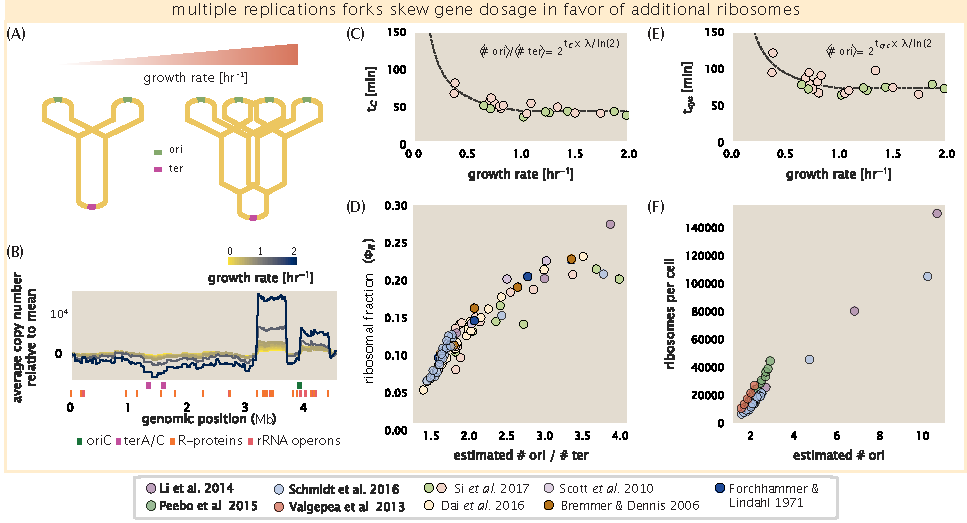
\includegraphics{main_figs/fig8_ribosome_growth_limit_ecoli_a.pdf}
        \caption{\textbf{Multiple replication forks skew gene dosage and
        ribosomal content.} (A) Schematic shows the expected increase in
        replication forks (or number of ori regions) as \textit{E. coli} cells
        grow faster. (B) A running boxcar average of protein copy number is
        calculated for each each growth condition considered by Schmidt
        \textit{et al.}. A 0.5 Mb averaging window was used. Protein copy
        numbers are reported relative to their condition-specific means in order
        to center all data sets. (C) and (E) show experimental data from Si
        \textit{et al.} (2017) Solid lines show fits to the data, which were
        used to estimate $\langle$\# ori$\rangle$ / $\langle$\# ter$\rangle$ and
        $\langle$\# ori$\rangle$ [NB: to note fit equations]. Red data points
        correspond to measurements in strain MG1655, while light green points
        are for strain NCM3722. (D) Plot compares our estimate of $\langle$\#
        ori$\rangle$ / $\langle$\# ter$\rangle$  to the experimental
        measurements of ribosomal abundance. Ribosomal fraction was approximated
        from the RNA/protein ratios of Dai \textit{et al.} (2016) (yellow) and
        Si \textit{et al.} (2017) (light red and light green) by the conversion
        RNA/protein ratio $\approx \Phi_R \cdot 2.1$. (F) Plot of the ribosome
        copy number estimated from the proteomic data against the estimated
        $\langle$\# ori$\rangle$.} \label{fig:translation_ecoli_partA}
    }
    \end{fullwidth}
\end{figure*}

If ribosomal genes (rRNA and ribosomal proteins) are being synthesized at
their maximal rate according to the rRNA gene dosage, we can make two related
hypotheses about how their ribosome abundance should vary with chromosomal
content. First, the ribosomal protein fraction should increase in proportion
to the average ratio of DNA origins to DNA termini ($\langle$\# ori$\rangle$
/ $\langle$\# ter$\rangle$ ratio). This is a consequence of the skew in DNA
dosage as cells grow faster. The second hypothesis is that the absolute
number of ribosomes should increase with the number of DNA origins
($\langle$\# ori$\rangle$), since this will reflect the total gene dosage at
a particular growth condition.

In order to test each of these expectations we considered the experimental data
from \cite{si2017}, which inferred these parameters for cells under
nutrient-limited growth. The ratio $\langle$\# ori$\rangle$ / $\langle$\#
ter$\rangle$ depends on how quickly chromosomes are replicated relative the
cell's doubling time $\tau$ and is given by 2$^{\tau_C / \tau}$. Here $\tau_C$
is the time taken to replicate \textit{E. coli}'s chromosome, referred to as the
C period of cell division.  In \FIG{translation_ecoli}(C) we plot the measured
$\tau_C$ versus $\tau$ (computed as $\tau = \log (2) / \lambda$), with data
points in red corresponding to \textit{E. coli} strain MG1655, and blue to
strain NCM3722. \cite{si2017} also measured the total RNA to protein ratio
which reflects ribosomal abundance and we show that data along with other recent
measurements from \cite{dai2016,dai2018}. Indeed, we find that the ribosomal
fraction increases with $\langle$\# ori$\rangle$ / $\langle$\# ter$\rangle$
(\FIG{translation_ecoli}(C)). We note a systematic difference in the relative
abundances from \cite{peebo2015} and \cite{valgepea2013} that was inconsistent
with a number of other measurements of total RNA-to-protein ratios ($\approx
\Phi_R$ x 2.1 \cite{dai2016}) and only show the data from \cite{schmidt2016} and
\cite{li2014} for relative ribosome abundances (see supplemental section XX for
a more complete discussion). For the data shown, the ribosomal fraction doesn't
increase as much at higher $\langle$\# ori$\rangle$ / $\langle$\# ter$\rangle$.
Since several rRNA operons are actually located approximately half-way between
the origin and terminus, the trend may in part be a consequence of a diminishing
increase in rRNA gene dosage at higher $\langle$\# ori$\rangle$ / $\langle$\#
ter$\rangle$ ratios.

We can similarly estimate $\langle$\# ori$\rangle$, which depends on how often
replication forks are initiated per cell cycle. This is given by the number of
overlapping cell cycles,  2$^{\tau_{cyc} / \tau}$, where $\tau_{cyc}$, refers to
the total time of chromosome replication and cell division.
\FIG{translation_ecoli}(E) shows the associated data from \cite{si2019},
which we use to estimate $\langle$\# ori$\rangle$  for each growth condition of
the proteomic data. In agreement with our expectations, we find that ribosome
copy number increases with the estimated $\langle$\# ori$\rangle$
(\FIG{translation_ecoli}(F)).

While it is difficult to distinguish between causality and correlation, the data
is at least consistent with the need for cells to increase their effective rRNA
gene dosage in order to grow according to the constraint set by Equation 2.
These results may also shed some light on the notable increase in ribosomal
content that is observed when sublethal doses of antibiotics \citep{scott2010,
dai2016}. Specifically, if rRNA synthesis is rate limiting, and nutrient
conditions largely dictate the extent of overlapping DNA replication cycles,
than addition of antibiotic will lengthen the doubling time and allow an
increased rRNA synthesis relative to the rate
of cell division. In Supplemental Section XX, we consider this further using
additional data from \cite{si2017}.

\subsection{Regulation of translating ribosomes helps maintain maximal growth
according to nutrient availability.}

While the above analysis provides a possible explanation for how \textit{E. coli}
can vary its ribosomal content to maximize growth, it also presents a
challenge in the limit of poorer nutrient conditions. Recall from Equation
\ref{eq:translation_limit_growth_rate} that ribosomal content should decrease to
zero as growth decreases to zero. While bacteria tend to decrease their
ribosomal abundance in poorer nutrient conditions, they do so only to some
fixed, non-zero amount \citep{scott2010, liebermeister2014}. Here we find a
minimal ribosomal fraction of $\approx$ 0.06 in the slowest growth conditions.
From the perspective of a bacterium dealing with uncertain nutrient conditions,
there is likely a benefit for the cell to maintain some relative fraction of
ribosomes to support rapid growth as nutrient conditions improve.

The challenge however, lies in the cell's ability to maintain steady-state
growth when ribosomes are in excess of the rate that nutrients can be harvested
and amino  acids synthesized for consumption \FIG{translation_ecoli}{G}. One
explanation for this is that the elongation rate decreases in poorer growth
conditions. Cells, however, are still able to maintain a relatively high
elongation rate even in stationary phase ($\approx$ 8 AA/s, \citep{dai2016,
dai2018}). A second explanation is that there are mechanisms to regulate
biological activity in conditions of stress and nutrient-limitation; in
particular through the small-molecule alarmones (p)ppGpp \citep{harris2018}.
Here we explore these two observations to better understand their consequence on
growth rate.

We consider slow growth conditions ($\lambda$ less than ~ 0.5 $hr^{-1}$) by
assuming that the decrease in elongation rate is due to a
limiting supply of amino acids and a need for the cell to maintain excess
nutrients for cellular homeostasis under steady-state growth. There is some
experimental support showing that in poorer nutrient growth conditions, cells
have lower amino acids concentrations \citep{bennett2009}. We proceed by coarse
graining the cell's amino acid supply as an single, effective rate-limiting
species (see Supplmental Section XX for a more complete discussion). Under such a scenario,
the elongation rate can described as simply depending on the maximum elongation
rate ($\approx$ 17.1 aa/s, \citep{dai2016, dai2018}), an effective $K_d$, and
the limiting amino acid concentration $[AA]_{eff}$. Specifically, the elongation
rate is given by,

\begin{equation}
r_t = r_t^{max} \cdot \frac{1}{1 + K_d / [AA]_{eff}}.
\label{eq:rate_Kd}
\end{equation}
For cells growing in minimal media + glucose, the amino acid concentration is of
order 100 mM  (BNID: 110093, \citep{milo2010, bennett2009}). With a growth rate
of about 0.6 hr$^{-1}$ and elongation rate of 12.5 aa per second
\citep{dai2016}, we can estimate an effective $K_d$ of about 40 mM. Ultimately
the steady state amino acid concentration will depend on the difference between
the supply of amino acids $r_{aa}$ and consumption by ribosomes $r_t \cdot R
\cdot f_a$, where $f_a$ accounts for the possible reduction of actively
translating ribosomes.

In \FIG{translation_ecoli}{E} we consider how the maximal growth rate and
elongation rates vary as a function of the number of actively translating
ribosomes in this slow growth regime (see Supplemental Section XX for a complete
description of the model). If we consider $r_{AA}$ to be reflective of a specific
growth condition, by considering lines of constant $r_{AA}$, we find that cells
grow fastest by maximizing their fraction of actively translating ribosomes.
When we consider the experimental measurements from \cite{dai2018}, we see
that although cells indeed reduce $R \times f_a$, they do so in a way that keeps
$[AA]_{eff}$ relatively constant. Given our estimate for the $K_d$ of 40 mM,  we
would only expect a decrease from 100 mM to about 35 mM in the slowest growth
conditions. While experimental data is limited, amino acid concentrations only
decrease to about 60 mM for cells grown in minimal media + acetate ($\lambda$ ~
0.3 hr$^{-1}$ in our proteomic data; value obtained from \cite{bennett2009}), qualitatively consistent with our expectations.

\begin{figure*}
    \begin{fullwidth}
    \centering{
        \includegraphics{main_figs/fig8_ribosome_growth_limit_ecoli_b.pdf}
        \caption{\textbf{\textit{E. coli} must regulate ribosomal activity in
        limiting nutrient conditions. }
        (A) Schematic showing translation-specific requirements for maintenance
        of steady-state growth. In a nutrient rich environment, amino acid
        supply $r_{aa}$ is sufficiently in excess of the demand by ribosomes
        translating at their maximal rate. In poorer nutrient conditions,
        reduced amino acid supply $r_{aa}$ will decrease the rate of elongation.
        In a regime where $r_{aa}$ is less than $r_t \cdot R$, the number of
        actively translating ribosomes will need to be reduced in order to
        maintain steady-state growth. (B) Translation elongation rate is plotted
        as a function of the number of actively translating ribosomes $R \cdot
        f_a$. Dashed lines correspond to a range of amino acid synthesis rates
        $r_{aa}$, from 10$^3$ to 10$^6$. Growth rates are calculated according
        to Equation 1, assuming a constant ribosomal fraction of 8 percent. See
        appendix XX for additional details. (C) Experimental data from Dai
        \textit{et al.} are used to estimate the fraction of actively
        translating ribosomes. The solid line represents the translation-limited
        growth rate for ribosomes elongating at 17.1 AA/s. }
        \label{fig:translation_ecoli_partB}
    }
    \end{fullwidth}
\end{figure*}

Given the quantitative data from \cite{dai2018}, which determined $f_a$
across the entire range of growth rates across our data, we next estimated the
active fraction of ribosomal protein. As shown in \FIG{translation_ecoli}(G), we
find that cells grow at a rate near the expected translation maximum expected
from Equation 1, using the maximum elongation rate of $r_t$ = 17.1 aa per
second. This is in contrast to the reality that ribosomes are translating at
almost half this rate in the poorest growth conditions. This highlights that
there are alternative ways to grow according to the translated-limited growth
rate that is expected based with ribosomes translating at their maximal
elongation rate. Specifically, it is by adjusting $r_t \times R \times f_a
\approx r_{tmax} \times R'$ that cells are able to scale the growth limit set by
Equation 2.

[NB, include in
discussion section: A number of recent papers highlight the possibility that
(p)ppGpp may even provide a causal explanation for the nutrient-limit scaling
law. In the context of ribosomal activity, increased levels of (p)ppGpp are
associated with lower ribsomal content, and at slow growth appear to help reduce
the fraction of actively translating ribosomes \citep{dai2016, dai2018}.
Titration of the cellular (p)ppGpp concetrations (up or down) can invoke similar
proteomic changes reminiscent of those observed under nutrient limitation
\citep{zhu2019}. In light of the limiting dependence of ribosome copy number on
chromosomal gene dosage, it was recently shown that growth in a (p)ppGpp  null
strain abolishes both the scaling in cell size  and the $\langle$\# ori$\rangle$
/ $\langle$\# ter$\rangle$ ratio. Instead, cells exhibited a high $\langle$\#
ori$\rangle$ / $\langle$\# ter$\rangle$ closer to 4 and cell size more
consistent with a fast growth state where (p)ppGpp levels are low
\citep{fernandezcoll2020}.]
